%\chapter{Terminology for frequency control service in different markets}
%\label{app:terminology-frequency-control}

\chapter{Data and Parameters for Quantitative Studies}
\chaptermark{Data and parameter}
\label{Appendix-data}
\textit{This appendix introduces the data preparation and parameter determination to render the model introduced in Chapter \ref{ch:methodology} to conduct quantitative studies in Section \ref{sec:quantitative}. We will introduce the sources of data and how the original data is pre-processed into inputs for the model as well as how the parameters of the model is set}

\section[Data and parameters for market-based modules]{Data and parameters for market-based modules%}
	\sectionmark{Market-based}}
\sectionmark{Market-based}
\label{sec:accounting-data-prepare}

Electricity market data, as we have seen clearly in Chapter \ref{ch:methodology}, is the crucial inputs for our model. It will be used both for direct valuation or as input to parameterize the market simulation module. In Chapter \ref{ch:LitRev}, we have argued that direct valuation using actual price is meaningful but only valid for the short rum. Therefore, we use the latest possible power market data by the time when this study was initiated, which corresponds to the actual market data from January 1st 2016 to December 31st 2016. The sources and preparation of power market data are introduced in the reminder of this section.

\subsection*{PJM}
All PJM electricity market data used in this study are retrieved from the official data management tool of PJM - Data Miner 2 \cite{Data_miner_2}. The sets of data used in this study are list in Table \ref{tab:pjm-data}.

\begin{table}
	\footnotesize
	\centering
	\begin{tabular}{L{5cm} L{2cm} L{6cm} }
		\hline
		\textbf{Data-set} & \textbf{Resolution} & \textbf{Description} \\
		\hline
		\hline
		Generation by Fuel Type & 15 min & Generation in MW for each fuel type, e.g. coal, hydro, wind, etc. \\
		\hline
		Hourly Day-Ahead Demand Bids & 1 hour & Aggregated hourly demand bids submitted to the Day-Ahead Energy Market, in MWh/h \\
		\hline
		Hourly Load: Metered & 1 hour & Actual load as consumed by the service territories within the PJM, in MWh/h \\
		\hline
		Day-Ahead Hourly LMPs & 1 hour & Hourly Day-Ahead Energy Market locational marginal pricing (LMP) data for all bus locations, including aggregates \\
		\hline
		Real-Time Hourly LMPs & 1 hour & Hourly Real-Time Energy Market locational marginal pricing (LMP) data for all bus locations, including aggregates\\
		\hline
		Ancillary Service Market Results & 1 hour & Hourly Ancillary service market results including MW quantities and prices\\
		\hline
		Regulation Market Data & 1 hour & Amount of Regulation that needs to be carried in the hour, adjusted by the effective MW, also including mileage ratios and overall performance scores \\
		\hline
		RTO Regulation Signal Data\footnote{This data set is not incorporated in Data Miner 2 but can be found at \url{http://www.pjm.com/markets-and-operations/ancillary-services.aspx}} & 2 second& Regulation control signal used within PJM RTO control area, including both RegD and RegA signals\\
		\hline
	\end{tabular}
	\caption{List of data sets used for PJM electricity market data}\label{tab:pjm-data}
\end{table}

In the reminder of this section, we will describe how these data are converted to the inputs for our model, with donations inheriting from what have been used in Chapter \ref{ch:methodology}.

First of all, the sets of marketplaces are defined as:

\begin{itemize}
	\item Set of energy marketplace $\mathbb{I} = \{1,2\}$:
	\begin{itemize}
		\item \textbf{1}: day-ahead market;
		\item \textbf{2}: real-time market.
	\end{itemize}
	\item Set of ancillary marketplace $\mathbb{J}=\{1,2\}$:
	\begin{itemize}
		\item \textbf{1}: regulation dynamic (RegD);
		\item \textbf{2}: regulation conventional (RegA).
	\end{itemize}
\end{itemize}

Preparation of price signals is related to the accounting rules\cite{PJM2017} so might be complicated especially for regulation price.

\subsubsection{Energy market price $\Pi_1$ and $\Pi_2$}

$\Pi_1$: Directly taken from \textit{Hourly Day-Ahead Demand Bids}.

$\Pi_2$:
Directly taken from \textit{Hourly Real-Time Demand Bids}.
\subsubsection{Frequency control price $\Phi_1$, $\Phi_2$, $\Psi_1$ and $\Psi_2$}

Firstly, the energy delivery is settled in real-time so:
\begin{equation*}
\Phi_1 = \Pi_1
\end{equation*}
\begin{equation*}
\Phi_2 = \Pi_1
\end{equation*}

The rest of service delivery is priced based on both the amount of capacity and actual perform, calculated from a list of factors including:

\begin{itemize}
	\item \textbf{Regulation Market Capacity Clearing Price (RMCCP)}: obtained from \textit{ Regulation Market Data}
	\item \textbf{Regulation Market Performance Clearing Price (RMPCP)}: obtained from \textit{ Regulation Market Data}
	%\item \textbf{Hourly-integrated Regulation (MW)}: adjusted by the effective MW, directly obtained from \textit{Regulation Market Data}
	\item \textbf{Actual Performance Score}: is defined as the measurement of accuracy, delay and precision. We use the overall performance for each service directly obtained from \textit{ Regulation Market Data}
	\item \textbf{Mileage Ratio}: is the absolute sum of movement of the regulation signal in a given time period. We use the overall mileage ratio for each service directly obtained from \textit{ Regulation Market Data}
	\item \textbf{Lost Opportunity Credit}: is the difference in net compensation from the Energy Market between what a resource. It is calculated only for resources providing energy along with regulation service so \$0 for non-energy regulation resources. Since none of the flexibility solutions studied quantitatively in this thesis are energy-providing resources, we exclude the lost opportunity credits from our optimization.
\end{itemize}

Thereby, the price signals are calculated as:

\begin{equation*}
\Psi_j = \left(\text{RMCCP} + \text{RMPCP} \times \text{Mileage Ratio}\right) \times \text{Actual Performance Score}
\end{equation*}
\begin{equation*}
\forall j \in \mathbb{J} =\{1,2\}
\end{equation*}

\subsubsection{Liquidity: market volumes $\hat{E}_1$, $\hat{E}_1$, $\hat{C}_1$ and $\hat{C}_2$}
Day-ahead market volume $\hat{E}_1$: is obtained directly from \textit{Hourly Day-Ahead Demand Bids}.

Real-time market volume $\hat{E}_2$: is calculated as the differences between actual metered load obtained from \textit{Hourly Load: Metered} and day-ahead market volume $\hat{E}_1$.

Regulation market volume $\hat{C}_1$ and $\hat{C}_2$: is obtained directly from \textit{Regulation Market Result} (including only pool-procured while excluding self-scheduled).

\subsubsection{Frequency control signal $\Delta_1$ and $\Delta_2$}
$\Delta_1$ and $\Delta_2$ are derived from the data-set \textit{RTO Regulation Signal Data} by binning the original signal to hourly blocks in order to comply with the time resolution of the model.

\subsubsection{Generation data $g_{f}$}

The generation data, $g_{f}$, and the sets of generation fuel types, $\mathbb{F}$, where $f \in \mathbb{F}$ are derived from the data-set \textit{Generation by Fuel Type}.  $g_{f}$ is calculated by binning the original signal to hourly blocks in order to comply with the time resolution of the model.

\subsubsection{Notice}
Credit for regulation services is calculated as the product of price and effective capacity. Effective capacity is determined as the nominal capacity multiplied by a so-called ``benefit factor". For RegA services, benefit factor is always 1 while for RegD the benefit factor is varying between 0 to 2.9 and is determined by the historical performance of a resource. For simplicity, we take the benefit factor being 1 as a system average level.
%NSW Generation
%https://www.aemo.com.au/Electricity/National-Electricity-Market-NEM/Planning-and-forecasting/Generation-information

%\subsubsection{Accounting}

%\subsection{Germany}


%$\pi_t^{e,i}, i \in \{Balancing\}$, is the the price for balancing energy (reBAP), which exist only in Germany

%$\pi_t^{r,j}$ and $\pi_t^{e,j}$ are based on principle of pay-as-bid. The weighted-average values are available in the datasets.


%Prices for balacning energy are unified across TSOs and determined according to the  balancing energy price settlement system (BK6-12-024) developed by Federal Network Agency (FNA) as of 01/12/2012.


%The unit prices of reserve products, $\pi_t^{r,j}$ and $\pi_t^{e,j}$, are not available in datasets published by AEMO. Only weekly summary for total payment and recovery are provided. Due to the limits of available data, we are only able to perform calculations of total potential revenues, rather than thorough studies as in the other two geographies.

\subsection*{DE}

The electricity market data for Germany is primarily retrieved from the official electricity market information platform ``SMARD" \cite{Smarde_web} managed by Bundesnetzagentur (BNetzA), the energy sector regulation in Germany. The platform publishes all data that is required by the Energy Industry Act (Energiewirtschaftsgesetz - EnWG) to be made freely available for public use. Meanwhile, the we refer to the website of EPEX SPOT for the day-ahead and intra-day market data, including price and volume. Data from BNetzA are listed in Table \ref{tab:DE-data}.

\begin{table}
	\footnotesize
	\centering
	\begin{tabular}{L{5cm} L{2cm} L{6cm} }
		\hline
		\textbf{Data-set} & \textbf{Resolution} & \textbf{Description} \\
		\hline
		\hline
		Electricity Generation - Actual Generation & 15 min & Generation in MWh for each fuel type, e.g. coal, hydro, wind, etc. \\
		\hline
		Electricity Consumption - Actual Consumption & 15 min & Consumption in MWh \\
		\hline
		Balancing energy & 15 min & Price (reBAP) in EUR/MWh and volume of balancing energy in MWh \\
		Primary control reserve & 15 min & Price\footnote{Prices for frequency control are determined using pay-as-bid scheme, so they are volume-averaged prices on a overall level.} for capacity in EUR/MW and total procured capacity in MW\\
		Secondary control reserve & 15 min & Price$^a$ for capacity in EUR/MW, price for energy in EUR/MWh, and total procured capacity in MW\\
		\hline
	\end{tabular}
	\caption{List of data sets used for DE electricity market data from BNetzA}\label{tab:DE-data}
\end{table}

In the reminder of this section, we will describe how these data are converted to the inputs for our model, with donations inheriting from what have been used in Chapter \ref{ch:methodology}.

First of all, the sets of marketplaces are defined as:

\begin{itemize}
	\item Set of energy marketplace $\mathbb{I} = \{1,2\}$:
	\begin{itemize}
		\item \textbf{1}: day-ahead market;
		\item \textbf{2}: real-time market;
		\item \textbf{3}: balancing market.
	\end{itemize}
	\item Set of ancillary marketplace $\mathbb{J}=\{1,2\}$:
	\begin{itemize}
		\item \textbf{1}: primary control reserve;
		\item \textbf{2}: secondary control reserve.
	\end{itemize}
\end{itemize}

\subsubsection{Energy market price $\Pi_1$, $\Pi_2$, and $\Pi_3$}

$\Pi_1$ and $\Pi_2$: Directly taken from EPEX SPOT website.

$\Pi_3$:
Directly taken from the data-set \textit{Balancing energy} from BNetzA

\subsubsection{Frequency control price $\Phi_1$, $\Phi_2$, $\Psi_1$ and $\Psi_2$}

All these items are taken from the data-sets \textit{Primary control reserve} and \textit{Second control reserve} from BNetzA. However, as mentioned in the table, it should be noted that these prices are pay-as-bid and what provided by BNetzA are the volume-averaged prices. We take the data from BNetzA as direct input, because the average prices on system-level suffice our needs of valuation for the whole market.

\subsubsection{Liquidity: market volumes $\hat{E}_1$, $\hat{E}_1$, $\hat{C}_1$ and $\hat{C}_2$}
Dealing with day-ahead market volume $\hat{E}_1$ is less straightforward. In the other two cases where electricity markets are organized in power pool arrangement and all electricity transactions would go through the day-ahead market gateway. Therefore, in order to make it comparable, we also use the total consumption from the data-set \textit{Consumption - Actual Consumption} as day-ahead market volume.

Intra-day market volume $\hat{E}_2$: is obtained from EPEX SPOT webstie

Volumes in balancing market  $\hat{E}_3$, primary control reserve $\hat{C}_1$ and secondary control reserve $\hat{C}_2$ are obtained directly from the data-sets from BNetzA.

\subsubsection{Frequency control signal $\Delta_1$ and $\Delta_2$}

No public data for control signals are found. Therefore, we take the ratio between total energy delivery and total committed capacity provided by the data-sets from BNetA as control signals $\Delta_1$ and $\Delta_2$. It should be noted that since the energy delivery for primary control reserve is not accounted for payments, $\Delta_1$ is virtually being 0 in our inputs.

\subsubsection{Generation data $g_{f}$}

The generation data, $g_{f}$, and the sets of generation fuel types, $\mathbb{F}$, where $f \in \mathbb{F}$ are obtained from \textit{Generation - Actual Generation} from BNetzA.

\subsection*{NSW}

The electricity market data is obtained on the website of Australian Energy Market Operator (AEMO) where the real-time market price and volume, as well as the total payment for ancillary service are available. However, there is not price (unit payment) data available for frequency control services, and for this reason wo do not carry out quantitative studies for frequency control services in th case of NSW. 

Therefore, there is only one marketplace studied so the set of marketplaces is defined as:

\begin{itemize}
	\item Set of energy marketplace $\mathbb{I} = \{1\}$:
	\begin{itemize}
		\item \textbf{1}: real-time market.
	\end{itemize}
\end{itemize}

\subsubsection{Real-time market price $\Pi_1$ and volume $\hat{E_1}$}

Both the price and volume data are available on AEMO's website so are used directly in our study. It should be noticed that the settlement time interval for the energy market in the case of NSW is half hour, compared to 1 hour for the other two cases.
%NSW Generation
%https://www.aemo.com.au/Electricity/National-Electricity-Market-NEM/Planning-and-forecasting/Generation-information

%\subsubsection{Accounting}





%The real-time market price is applied for all deviations from day-ahead planned schedule, including Regulation, Primary and Supplementary Reserves.

%\begin{equation*}
%\pi_t^{e,j} = \pi_t^{e,i} ~~~~ i \in \{Real~Time\}, j \in \{RegD, RegA, SR, NSR, DASR\}
%\end{equation*}

%The capacity prices of reserves are computed using a complex algorithm, taking into account a list of specifications of the resource, e.g. the performance \& historical performance, benefits factor, mileage, etc. The detailed calculations can be found in appendix. As outputs, we will get deterministic values for $j \in \{RegA, SR, NSR, DASR\}$, and the upper and lower bounds, $\overline{\pi}_t^{r,j}$ and $\underline{\pi}_t^{r,j}$, for $i \in \{RegD\}$.

%Reg = RMCCP + RMPCP + LOC
%LOC = 0
%RMCCP = 
%RMPCP = Milleage
%Effective MW = BF * MW
%BF is determined with the average and upper, lower bounds

\section[Data and parameters for technology-based modules]{Data and parameters for technology-based modules%}
	\sectionmark{Technology-based}}
\sectionmark{Technology-based}
\label{app:tech}

For the ideal storage system for estimating maximum market potential, the only parameter needs to be defined is the energy-to-power ratio, which indicates the maximum duration of a single continuous process of service provision. We use 8-hour that is a reasonable upper bound among all energy storage and load-shifting technologies \cite{Muller2016}. We ignore all possible losses, i.e. all efficiencies are assumed to be 1 for the ideal storage system.

In contrast, we model the losses for specific technologies, i.e. the battery energy storage system and electric vehicle to grid. The parameters are determined as shown in Table \ref{tab:battery-efficiency}. 

\begin{table}
	\centering
	\begin{tabular}{l r}
		\hline
		\textbf{Items} & \textbf{Value} \\% & \textbf{Reduced Cost} \\
		%\hline
		\hline
		Storage efficiency, $\eta^s$ & 100\% \\
		Discharge efficiency, $\eta^+$ & 96\% \\
		Charge efficiency, $\eta^-$ & 96\% \\
		\hline		
	\end{tabular}
	\caption{Battery efficiencies for modeling battery energy storage system and electric vehicle to grid}\label{tab:battery-efficiency}
\end{table}

With the discharge and charge efficiencies being 96\%, the round-trip efficiency is 92\% which corresponds to the numbers indicated in the literature \cite{Akhil2015,Megel2017,IRENA2017}. Besides, the energy-to-power ratio is taken as 4-hour as a typical value referring to the literature \cite{Muller2016,IRENA2017}.

Regarding cost determination, operational costs are same for BESS and EV2G due to the physical process is identical. However, as mentioned in Section \ref{sec:cost}, we do not account fixed costs for EV2G.

Cost parameters are first determined based on the present market pricing level. Scenarios with reduced costs will be made in certain cases to find the break-even point if it is not yet profitable. According to the International Renewable Energy Agency (IRENA) \cite{IRENA2017}, the cost for battery energy storage systems was analyzed as proportional to their energy capacity, $\overline{s}$, and the energy cost coefficient, $C^s$, for state-of-the-art lithium-ion batteries were reported to be ca. $\$350/kWh$ in 2016. The replacement cost were based on actual price from Tesla \cite{Tesla1}. The operating life is set to be 6000 FCEs, which corresponds to an optimistic estimation by Sandia National Laboratories \cite{Akhil2015}. Designed life time is assumed to be 10 years. Discount rate is made as 10\% as is discussed in Section \ref{sec:cost}. All the parameters for cost calculation are summarized in Table \ref{table:cost-parameters}. 

\begin{table}[h!]
	\begin{center}
		\begin{tabular}{ l  l  R{2.7cm} } %R{2.7cm} |}
			\hline
			\textbf{Items} & \textbf{Unit} & \textbf{Value} \\% & \textbf{Reduced Cost} \\
			%\hline
			\hline
			Energy cost coefficient, $C^s$ & $\$/kWh$ & 350 \\%& 140 \\
			%\hline
			Power cost coefficient, $C^r$ & $\$/kW$ & 0\\% & 0 \\
			%\hline
%			Technology cost, $C^0$ &$\$$ & 0\\% &0\\
			%\hline
			Replacement cost coefficient, $C^s$ &$ \$/kWh$ & 150\\% & 60 \\
			%\hline
			Designed life time & \textit{year} & 10\\% \multicolumn{2}{c|}{10}\\
			%\hline
			Operating life time & \textit{FCE} & 6000\\% \multicolumn{2}{c|}{6000}\\
			%\hline
			Discount rate &$\%$ & 10\\% \multicolumn{2}{c|}{10}\\
			\hline
		\end{tabular}
	\end{center}
	\caption{Parameters for cost calculation}\label{table:cost-parameters}
\end{table}

%It is worthwhile to emphasize that by using the parameters described above, the ESSs are essentially battery energy storage systems. The conclusions on profitability are not portal for other types of ESSs, not to say other types of flexibility solutions in a broader sense. However, the value of revenue that is independent from these cost terms should still be valid for other types of technologies.

For EV2G studies, we need to specify more parameters. Firstly, the model for a single EV is determined as:

\begin{itemize}
	\item EV charging rate is 10kW, corresponding to the guidance provided by Tesla\cite{Tesla2} and a typical home charging infrastructure with 50A current limit. 
	\item The battery energy capacity per EV of 75kWh is taken from one of the most popular EV models\cite{Tesla3}.
\end{itemize}

Simulations are then performed to get EV driving profiles, which are based upon data from the California Department of Transportation's California Household Travel Survey for 2010-2012\cite{NREL_TSDC}. This survey carried out multiple objectives and included 79011 vehicles. For our work we focus on a proportion of the vehicles, 2910, which were fitted with GPS. These vehicles were monitored continuously for a 7-day window with the 1-second resolution. The GPS data is then processed into trip profiles, while include information of the location of each vehicle at each time step as well as the trips made by each vehicle. While vehicles surveyed are not only electric vehicle but also other types of vehicles using internal combustion engines, we assume their driving patterns are similar. Such a assumption should be generally valid since it is not likely that users will alter their driving behavior if they switch from a conventional car to a EV. 

Further with the parameters of the EV model we have selected above we simulated the SoC time series of the EV batteries. Finally, from the simulated results, we can statistically derive the value of probability distribution of EV plug-in $n^+$, plug-out $n^-$, and average state-of-charge (SoC) of batteries plug-in $s^+$, plug-out $s^-$, as introduced in Section \ref{sec:tech-simulation-module}. The results are shown as Figure \ref{fig:data-ev-number}-\ref{fig:data-soc} where we can see clear periodic patterns that are different between weekdays and weekends.

\begin{figure}[h!]
	\centering
	\centering
	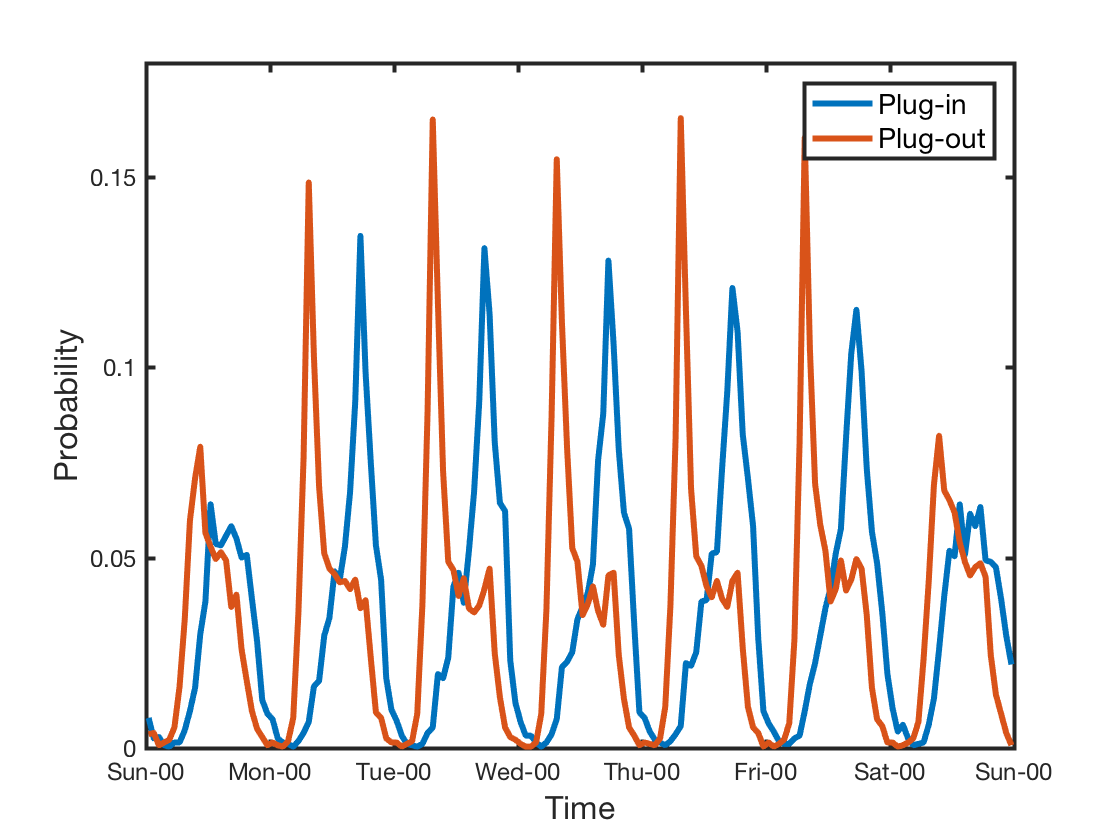
\includegraphics[width=0.8\linewidth]{Figures/Data_EV_number}
	\caption{Probability of EV plug-in/ plug-out}
	\label{fig:data-ev-number}
\end{figure}

\begin{figure}[h!]
	\centering
	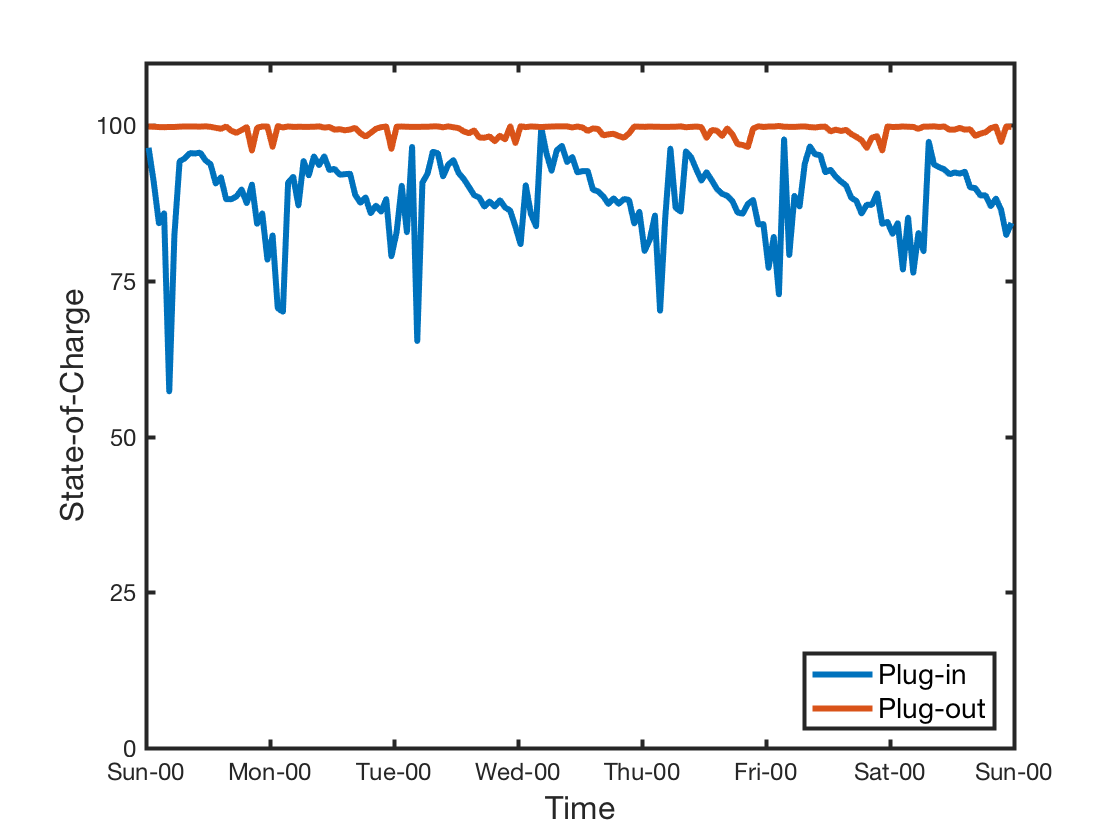
\includegraphics[width=0.8\linewidth]{Figures/Data_SoC}
	\caption{Average SoC of EV when plug-in/ plug-out}
	\label{fig:data-soc}
\end{figure}

Regarding the number of EV, we primarily refer to the official statistic for vehicle registration in Germany provided by the Federal Motor Transport Authority of Germany (Kraftfahrt-Bundesamtes, KBA)\cite{KBA2017}. Since the EV registered before 2010 is negligible, we conceived the cumulative registration since 2010 as the total number of EVs in Germany, shown as Figure \ref{fig:Germany_EV_number}. Besides, the total vehicle number in Germany is 45 million according to \cite{Eurostat_de_v}. We would refer to this number as well for scenario analysis.

\begin{figure}[h!]
	\centering
	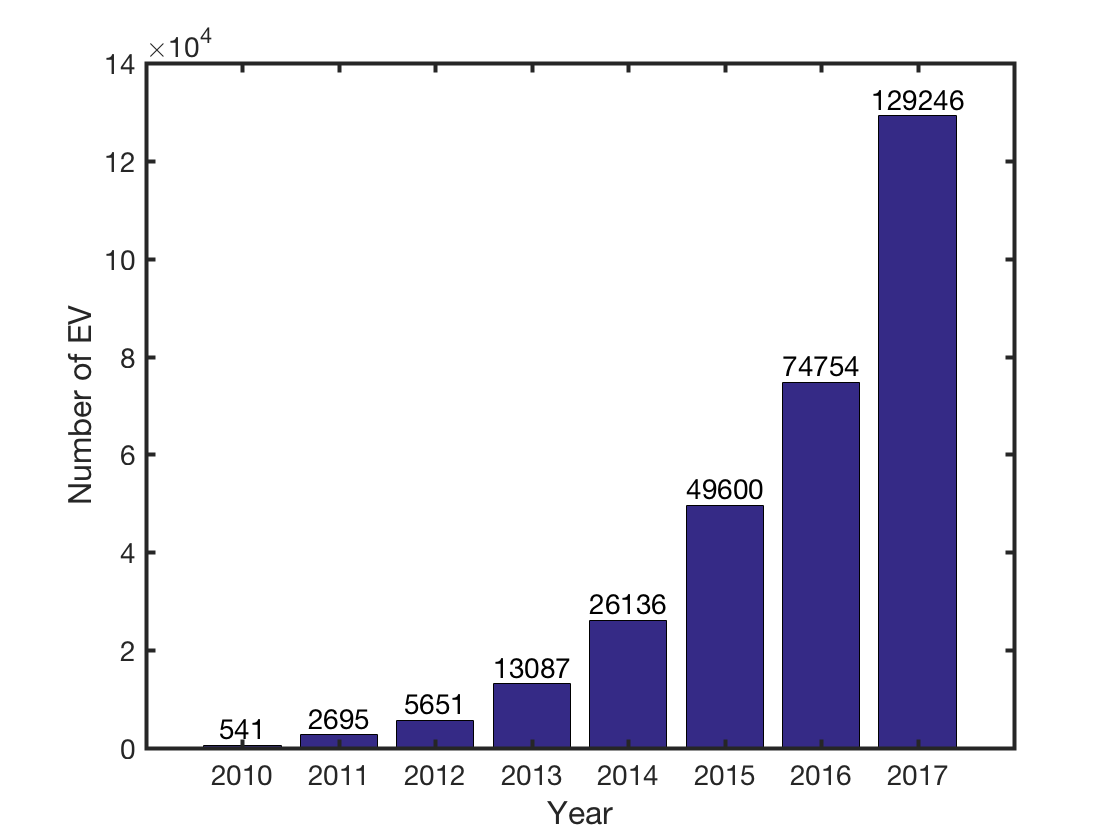
\includegraphics[width=0.95\linewidth]{Figures/Germany_EV_number}
	\caption{Cumulative registration of plug-in electric vehicles in Germany since 2010 \cite{KBA2017}}
	\label{fig:Germany_EV_number}
\end{figure}

There are no reliable data found for PJM, because its geographic coverage is not strictly corresponding to the administrative divisions. It is an extremely sophisticated task to get the official number of EVs with the public data. Therefore, we projected the number in Germany to PJM by their ratio of household number. That means, in the corresponding scenarios, the EV ownership per household is identical in Germany and PJM. We further applied the same exercise for EV number in NSW. In this way, we actually reduce one layer of complexity that is caused by different EV penetration rate in different regions so that we can keep focused on the characteristics of power markets, which is our main purpose of this study. Such a approach is taken to make some indications of the market values, which however shall be noticed with caution that it may deviate from real conditions. 










